\documentclass[a4paper,twoside]{book}

\usepackage[utf8]{inputenc}
\usepackage[english,russian]{babel}
\usepackage{fontspec}
\setmainfont{Liberation Serif}
\setmonofont{Liberation Mono}

\usepackage{graphicx}
\renewcommand{\thefigure}{\thesection.\arabic{figure}}
\usepackage{hyperref}
\usepackage{multirow}
\usepackage[absolute,overlay,showboxes]{textpos}
\usepackage{etoolbox}
\usepackage{longtable}
\usepackage{tikz}
\usepackage{lilyglyphs}
\usepackage{tabularx}
\usepackage{pgfplots}
\usepackage{circuitikz}
\usepackage{minted}
\usepackage{glossaries}

\makeglossaries

\usepackage{svg}

\urlstyle{same}
\usepackage[printonlyused,withpage]{acronym}

\graphicspath{ {images/} {../images/} }

%% \documentclass[../main.tex]{subfiles}
%% \usepackage{svg}
%% \graphicspath{{\subfix{../images/}}}
%% \begin{document}

\newcounter{example-counter}
\setcounter{example-counter}{1}

%% This procedure adds the "Example" block to the text.
\newcommand{\example}[1]{
  \vspace{8pt}
  \begin{tabularx}{\textwidth}{m{1cm} m{9cm}}
    \includesvg[width=1.25cm]{the-noun-project/request-mirrored}
    & \textbf{Пример \arabic{example-counter}}: #1 \\
  \end{tabularx}
  \addtocounter{example-counter}{1}
}

\newcounter{experiment-counter}
\setcounter{experiment-counter}{1}

%% This procedure adds the "Experiment" block to the text.
\newcommand{\experiment}[2]{
  \vspace{8pt}
  \begin{tabularx}{\textwidth}{m{.15\textwidth}X m{.85\textwidth-4}X}
    \includesvg[width=1cm]{the-noun-project/flask}
    & \textbf{Эксперимент №\arabic{experiment-counter}:} #2 \\
  \end{tabularx}
  \addtocounter{experiment-counter}{1}
}

\newcommand{\note}[1]{
  \vspace{8pt}
  \begin{tabularx}{\textwidth}{m{1cm} m{9cm}}
    \includesvg[width=1cm]{the-noun-project/note}
    & \textbf{Примечание:} #1 \\
  \end{tabularx}
}

\newcommand{\hotkey}[1]{
  \texttt{#1}
}

%% This procedure allows to insert a music note.
%% Syntax:
%%   \musicnote{<octave>}{<note-name>}{<frequency>}
\newcommand{\musicnote}[3]{
  &
  \ifstrequal{#2}{C}{До   & C#1}{}
  \ifstrequal{#2}{D}{Ре   & D#1}{}
  \ifstrequal{#2}{E}{Ми   & E#1}{}
  \ifstrequal{#2}{F}{Фа   & F#1}{}
  \ifstrequal{#2}{G}{Соль & G#1}{}
  \ifstrequal{#2}{A}{Ля   & A#1}{}
  \ifstrequal{#2}{B}{Си   & B#1 (H#1)}{}
  & #3 \\
}

%% Taken from:
%%   <https://tex.stackexchange.com/questions/184923/how-to-include-a-second-file-only-if-environment-variable-is-set>
\newcommand{\newgetenv}[2][]{%
 \CatchFileEdef{\temp}{"|kpsewhich --var-value #2"}{\endlinechar=-1\relax}%
 \if\relax\detokenize{#1}\relax\temp\else\edef#1{\temp}\fi%
}%

\newcommand\esymbol[1]{%
  \begin{circuitikz}%
    \draw (0,0) to [#1] (1,0);%
  \end{circuitikz}%
}

\newcommand*{\soundWaveIcon}[0]{%
  \begin{tikzpicture}
    \draw[black, fill=black] (0, 0) circle (.25mm);
    \draw (.5mm, 0.7mm) arc (45:-45:1mm);
    \draw (1mm, 1mm) arc (45:-45:1.5mm);
    \draw (1.5mm, 1.3mm) arc (45:-45:2mm);
  \end{tikzpicture}%
}

%% \end{document}


\usepackage{subfiles}

%%%%%%%%%%%%%%%%%%%%%%%%%%%%%%%%%%%%%%%%%%%%%%%%%%%%%%%%%%%%%%%%%%%%%%%%%%%%%%%%
\title{Автомато-программато-компарадио-кружок}
\author{Артём ``avp'' Попцов\\\href{https://memory-heap.org}{memory-heap.org}}
\input{version.tex}

\begin{document}

\maketitle

\tableofcontents

%%%%%%%%%%%%%%%%%%%%%%%%%%%%%%%%%%%%%%%%%%%%%%%%%%%%%%%%%%%%%%%%%%%%%%%%%%%%%%%%
\chapter*{Вступление}
\addcontentsline{toc}{chapter}{Вступление}

\subfile{sections/introduction.tex}

%%%%%%%%%%%%%%%%%%%%%%%%%%%%%%%%%%%%%%%%%%%%%%%%%%%%%%%%%%%%%%%%%%%%%%%%%%%%%%%%
\chapter{Основные принципы электротехники}

В первую очередь нам с вами надо рассмотреть базовые принципы того, как работает
электроника, чтобы впоследствии уметь собирать простые схемы.

Начнём с рассмотрения условий, которые необходимо выполнить, чтобы через
электрическую цепь шёл ток.

\subfile{sections/electronics-voltage}

\subfile{sections/electronics-circuits}

\subfile{sections/electronics-potential-difference}

\subfile{sections/electronics-resistance}

\subfile{sections/electronics-building-circuits}

%%%%%%%%%%%%%%%%%%%%%%%%%%%%%%%%%%%%%%%%%%%%%%%%%%%%%%%%%%%%%%%%%%%%%%%%%%%%%%%%
\chapter{Диалоги с компьютером}
\label{chapter:dialogues-with-computer}

\begin{figure}[ht]
  \centering
  \begin{tikzpicture}
    %% Display.
    \node[rectangle,
      rounded corners = 0.2,
      draw = black,
      minimum width = 3cm,
      minimum height = 2cm] (r) at (1, 2) {Hello, World!};

    \node[rectangle,
      thick,
      rounded corners = 0.25cm,
      draw = black,
      minimum width = 4cm,
      minimum height = 3cm] (r) at (1.25, 2) {};

    %% Display Knobs.
    \node[circle, draw, radius = 0.1cm] (c) at (2.85, 2.0) {};
    \node[circle, draw, radius = 0.1cm] (c) at (2.85, 1.6) {};
    \node[circle, draw, radius = 0.1cm] (c) at (2.85, 1.2) {};

    %% Display Legs.
    \node[rectangle,
      thick,
      draw = black,
      minimum width = 0.2cm,
      minimum height = 0.19cm] (r) at (0, 0.38) {};

    \node[rectangle,
      thick,
      draw = black,
      minimum width = 0.2cm,
      minimum height = 0.19cm] (r) at (2.25, 0.38) {};

    %% System Case.
    \node[rectangle,
      thick,
      rounded corners = 0.25cm,
      draw = black,
      minimum width = 5.5cm,
      minimum height = 1.5cm] (r) at (0.75, -0.48) {};

    %% Floppy Drives.
    \node[rectangle,
      draw = black,
      minimum width = 2cm,
      minimum height = 1.25cm] (r) at (2.25, -0.36) {};

    \node[rectangle,
      draw = black,
      minimum width = 1.75cm,
      minimum height = 0.5cm] (r) at (2.25, -0.1) {};

    \node[rectangle,
      draw = black,
      minimum width = 1.75cm,
      minimum height = 0.5cm] (r) at (2.25, -0.6) {};

    \draw[very thick] (1.5, -0.15) -- (3, -0.15);

    \draw[very thick] (1.8, -0.6) -- (2.7, -0.6);

    %% Control buttons.
    \node[rectangle,
      draw = black,
      minimum width = 1cm,
      minimum height = 0.25cm] (r) at (-0.4, -0.25) {};

    %% Ventilation holes in the case.
    \foreach \offset in {0.1, 0.2, ..., 2.6} {
      \draw[thick] (-1.8 + \offset, -1) -- (-1.8 + \offset, -0.5);
    };

  \end{tikzpicture}
\end{figure}

\subfile{sections/dialogues-with-computer-introduction}

\subfile{sections/dialogues-with-computer-algorithms}

\subfile{sections/dialogues-with-computer-arduino}

%%%%%%%%%%%%%%%%%%%%%%%%%%%%%%%%%%%%%%%%%%%%%%%%%%%%%%%%%%%%%%%%%%%%%%%%%%%%%%%%
\section{Работа с макетной платой}

Макетная плата позволяет собирать схемы (подключать электронику) без применения
пайки --- это упрощает прототипирование и ускоряет процесс разработки проектов.
Компоненты просто вставляются в слоты на макетной плате для соединения
(см. рис. \ref{fig:breadboard-led}.)

\begin{figure}[ht]
  \centering
  \caption{Пример подключения светодиода к Arduino Mega 2560 через макетную
    плату.}
  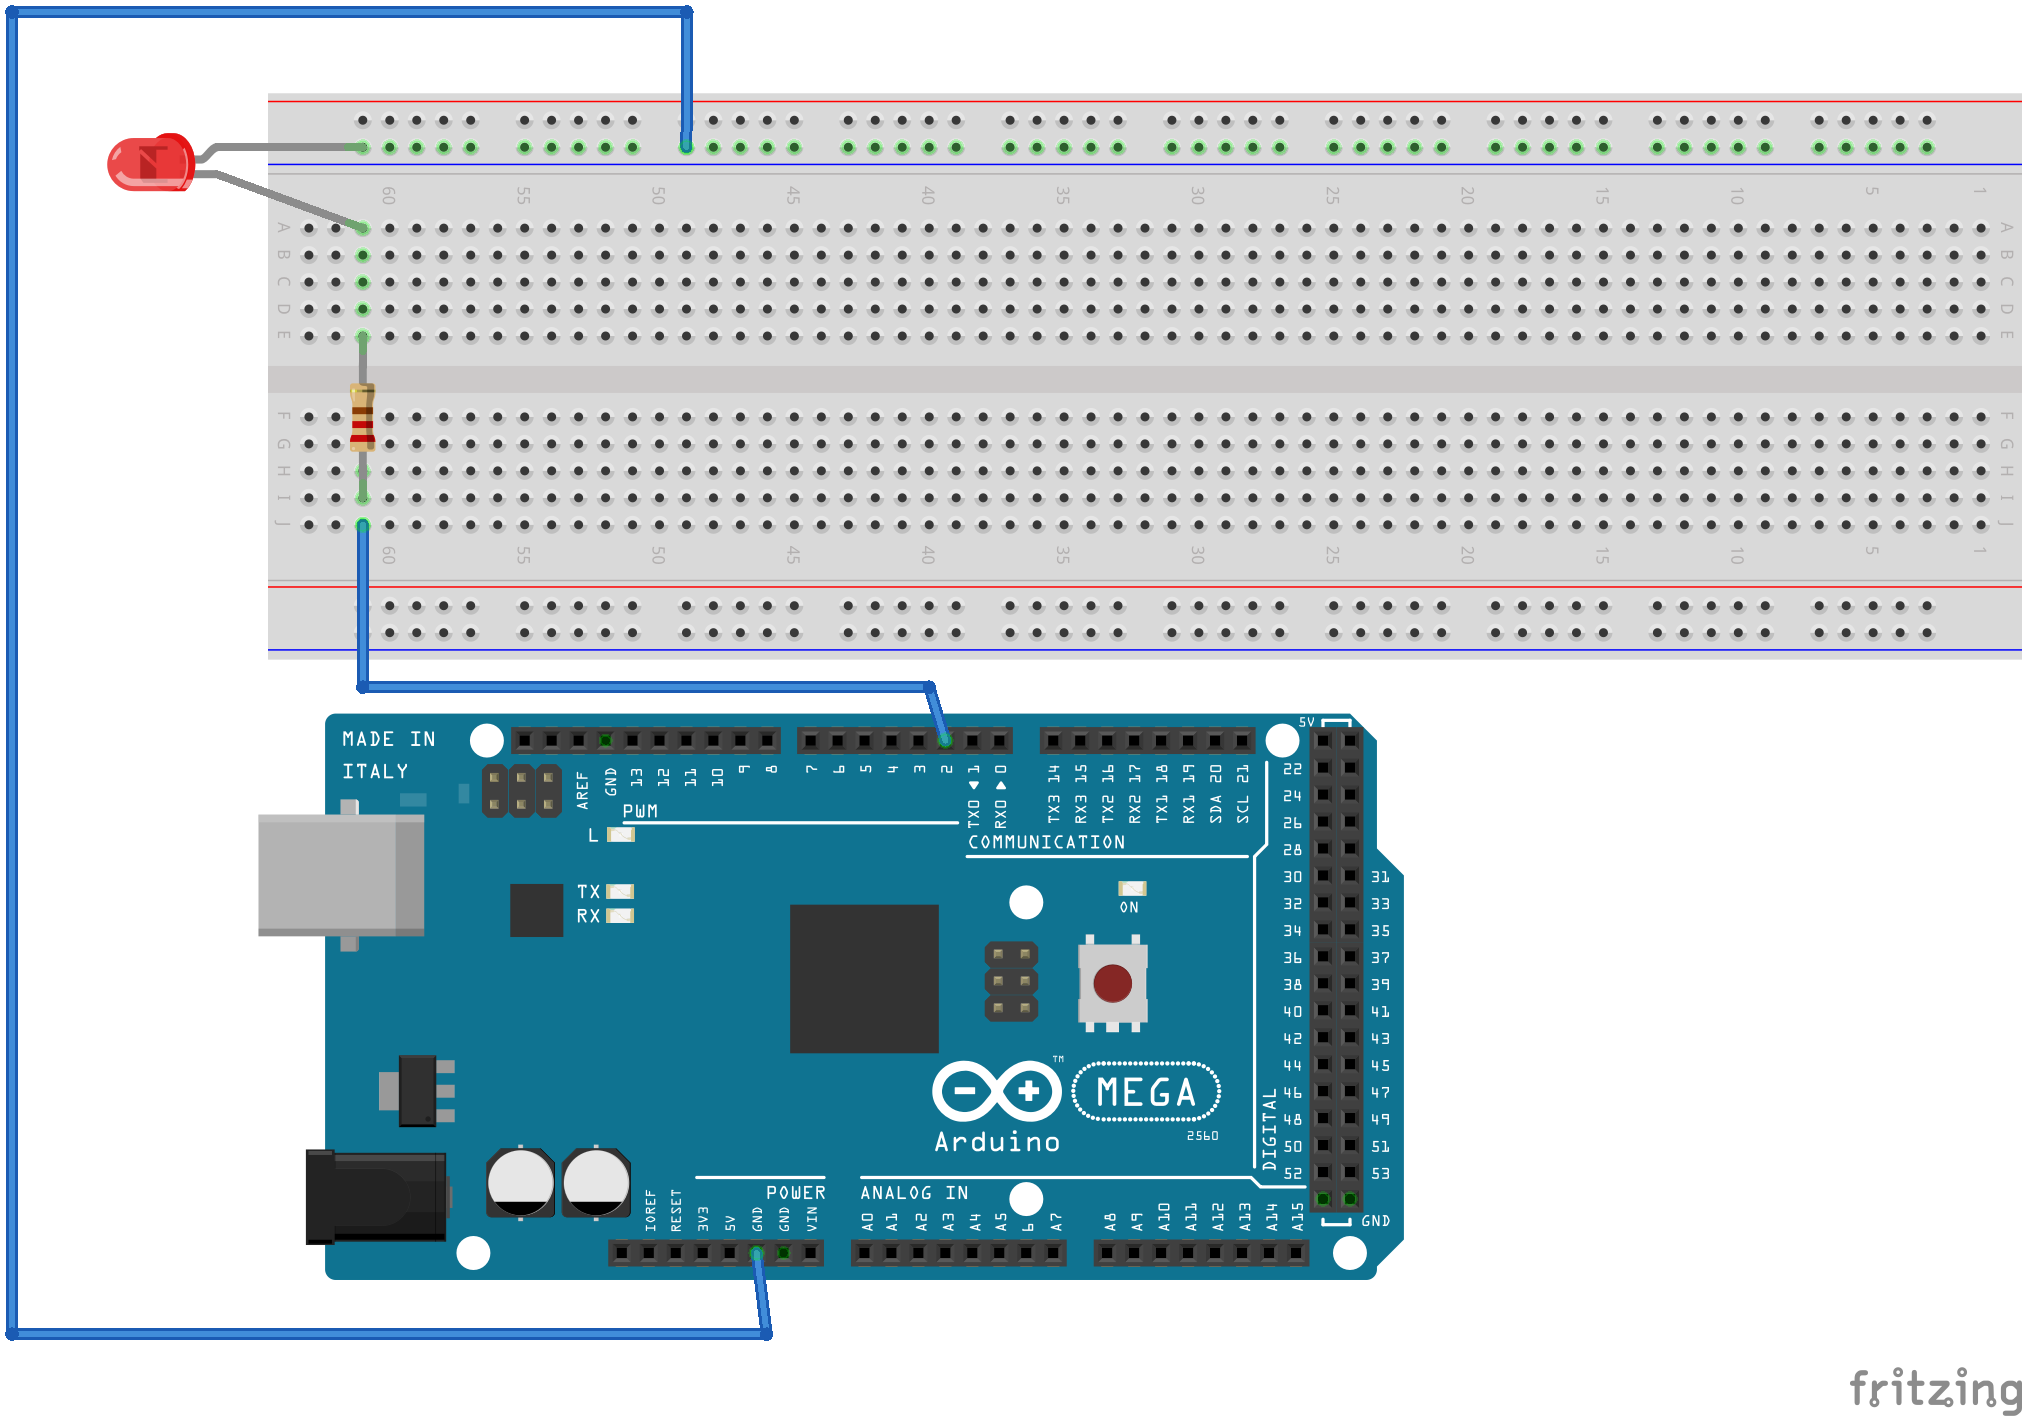
\includegraphics[width=12cm]{schematics/001-led}
  \label{fig:breadboard-led}
\end{figure}

\begin{itemize}
\item Черный провод подключен к arduino и идёт на вывод GND (минус)
\item Синий провод подключен к arduino и идёт на вывод 5V (плюс)
\end{itemize}

\note{ Обратите внимание, что светодиоды (и некоторые другие элементы)
  подключаются к платформе Arduino через резистор -- это необходимо для
  обеспечения бесперебойной работы схемы и предупреждения всяческих поломок и
  ухудшения работы как отдельных деталей, так и схемы в целом.  }

\section{Подключение Arduino к компьютеру}
Чтобы подключить ардуино к компьютеру вам потребуется сама платформа Arduino (в
нашем случае мы используем Arduino Mega 2560) и кабель стандарта USB-В.

Соедините Arduino с компьютером через USB-кабель. Вы увидите, как на плате
загорится светодиод ``ON''.

Теперь необходимо настроить Arduino IDE для работы с подключенной Arduino, для
этого нужно войти в панель ``Инструменты'' затем ``Плата'' -- в этом меню
выберите 6Arduino с которой вы сейчас работаете, затем в подменю ``Порт''
выберите порт, к которому подключена Arduino.

\newpage
\subfile{sections/dialogues-with-computer-arduino-ide}

\subfile{sections/dialogues-with-computer-program-structure}

\subfile{sections/dialogues-with-computer-memory}

\subfile{sections/dialogues-with-computer-control-flow}

%%%%%%%%%%%%%%%%%%%%%%%%%%%%%%%%%%%%%%%%%%%%%%%%%%%%%%%%%%%%%%%%%%%%%%%%%%%%%%%%
\chapter{Белый шум}

\subfile{sections/white-noise-introduction}
\subfile{sections/white-noise-signal-types}
\subfile{sections/white-noise-serial-port}
\subfile{sections/white-noise-analog-ports}
\subfile{sections/white-noise-adc}

%%%%%%%%%%%%%%%%%%%%%%%%%%%%%%%%%%%%%%%%%%%%%%%%%%%%%%%%%%%%%%%%%%%%%%%%%%%%%%%%
\chapter{Широтно-импульсная модуляция}

\subfile{sections/pwm-intro}
\subfile{sections/pwm-wavelength}
\subfile{sections/pwm-duty-cycle}


%%%%%%%%%%%%%%%%%%%%%%%%%%%%%%%%%%%%%%%%%%%%%%%%%%%%%%%%%%%%%%%%%%%%%%%%%%%%%%%%
\subsection{Задачи}

\begin{enumerate}
\item Написать программу, плавно включающую и выключающую светодиод. Собрать и
  протестировать схему. 
\item Написать программу, реализующую ``бегущий огонь'' с использованием ШИМ.
  Собрать и протестировать схему.
\item Используя потенциометр, модифицировать систему из задания №2 таким
  образом, чтобы можно было регулировать яркость ``бегущего огня''.
\item Разработать ``бегущий огонь'', где следующий светодиод начинает плавно
  разгораться одновременно с затуханием предыдущего светодиода.
\end{enumerate}

%% \section{Последовательный порт}

%% \subsection{Сбор и обработка данных на стороне компьютера}

%% Другой задачей, решаемой с помощью функций записи данных в последовательный
%% порт, является сбор данных на стороне компьютера. Arduino IDE позволяет нам
%% визуализировать данные через специальный плоттер (доступ к которому можно
%% получить, выбрав в меню ``Инструменты'' пункт ``Плоттер по последовательному
%% соединению'', либо нажав комбинацию клавиш \hotkey{Ctrl + Shift + L}.)

%% \subsection{Передача данных с компьютера на Arduino}

%% Передавать данные с Arduino на компьютер мы уже научились. Теперь посмотрим на
%% передачу данных в обратном направлении. Для того чтобы передать данные с
%% компьютера на Arduino также необходимо выполнить настройку последовательного
%% порта; кроме этого, нам потребуется задействовать несколько новых функций.

%% \subsubsection{Чтение отдельных байт}

%% Функция \texttt{Serial.read} читает байт данных из поступивших на Arduino. То
%% есть возвращает вам некое целое число, с которым вы вольны делать что вашей душе
%% угодно. Каждый вызов этого метода будет возвращать вам следующий байт данных из
%% тех что поступили на Arduino. Если возвращать нечего, то есть вы считали все что
%% было, данная функция вернет -1.

%% \note{ Если передаются именно байты, возникает проблема: -1 это 0xFF в
%%   шестнадцатиричной системе, или 255 в десятичной. Такой же байт, как и все
%%   остальные, из-за чего невозможно. поэтому нужно сперва вызывать функцию available . }

%% Допустим мы отправили 1 байт данных на Arduino и использовали нижеприведенный
%% участок кода:

%% \begin{verbatim}
%% int incoming_byte;
%% void loop() {
%%   if (Serial.available() > 0) {
%%       incoming_byte = Serial.read();
%%   }
%% }
%% \end{verbatim}

%% После того, как вы считаете байт данных, он будет перемещен в вашу переменную
%% \texttt{incoming\_byte} а функция \texttt{Serial.available} снова будет
%% возвращать 0, пока не поступят новые данные.

%% То есть, когда вы считываете байт, показания счетчика принятых байт уменьшается
%% и \texttt{Serial.available} будет показывать на 1 байт меньше.

%% Помните, что функция \texttt{Serial.read} возвращает только 1 байт данных, если
%% например вы передали 4 символа каждый по 1 байту, вам потребуется 4 раза вызвать
%% данную функцию чтобы прочитать эти символы и самостоятельно позаботится о том
%% чтобы разместить их в массив символов либо воспользоваться функцией
%% \texttt{Serial.readBytes}.

%% \subsubsection{Чтение чисел}

%% Функция \texttt{Serial.parseInt} просматривает данные, поступившие на Arduino, и
%% ищет среди них набор кодов (чисел) от 48 до 57, которые соответствуют символам
%% чисел от 0 до 9 и преобразует все это в правильное целочисленное значение. Таким
%% образом если вы с монитора порта передадите "число" (на самом деле, строку)
%% ``72'', данный метод увидит 2 последовательных байта 55 и 51, корректно
%% преобразует его в число 72 и вернет его как правильное целочисленное значение.
%% Давайте напишем маленькую эхо-программу, которая покажет принцип работы данной
%% функции и позволит вам узнать какому символу соответствует то или иное число.

%% \begin{verbatim}
%% int incoming_int = 0;

%% void setup()
%% {
%%   Serial.begin(9600);
%%   Serial.setTimeout(2000);
%% }
%% void loop()
%% {
%%   if (Serial.available() > 0)
%%   {
%%     incoming_int = Serial.parseInt();
%%     Serial.write(incoming_int);
%%   }
%% }
%% \end{verbatim}

%% Данная программа будет работать так. Если в мониторе порта вы введете строку
%% ``72'' то монитор порта отправит его на Arduino как два байта данных в виде
%% чисел 55 и 51, функция \texttt{Serial.parseInt} подождет 2000 миллисекунд (как
%% видите я поменял время ожидание с 1 секунды на 2 секунды, чтобы нагляднее
%% показать кое какие аспекты) увидит эти два значения и преобразует их в одно
%% целочисленное 72 и присвоит его переменной \texttt{incoming\_int}, мы с помощью
%% метода \texttt{Serial.write} передадим число 72 как есть обратно в монитор порта
%% (почему именно этот метод нужен читайте далее) где монитор порта корректно
%% преобразует число 72 в соответствующий символ и покажет нам символ ``H'' который
%% соответствует коду 72. Таким образом мы можем передавать числовые значения с
%% компьютера на платформу Arduino и дальше использовать эти значения.

\chapter{Синтез музыки и технологии}

\subfile{sections/music-and-technology-synthesis-sound}
\subfile{sections/music-and-technology-synthesis-speaker}
\subfile{sections/music-and-technology-synthesis-rhythm}
\subfile{sections/music-and-technology-synthesis-harmony}
\subfile{sections/music-and-technology-synthesis-octave-system}
\subfile{sections/music-and-technology-synthesis-simple-melodies}
\subfile{sections/music-and-technology-synthesis-arrays}
\subfile{sections/music-and-technology-synthesis-two-dimensional-arrays}
\subfile{sections/music-and-technology-synthesis-rest}
\subfile{sections/music-and-technology-synthesis-dotted-notes}
\subfile{sections/music-and-technology-synthesis-flats-and-sharps}
\subfile{sections/music-and-technology-synthesis-musical-scale}
\subfile{sections/music-and-technology-synthesis-bass-clef}

%%%%%%%%%%%%%%%%%%%%%%%%%%%%%%%%%%%%%%%%%%%%%%%%%%%%%%%%%%%%%%%%%%%%%%%%%%%%%%%%
\addcontentsline{toc}{chapter}{Словарь терминов}
\printglossaries

%%%%%%%%%%%%%%%%%%%%%%%%%%%%%%%%%%%%%%%%%%%%%%%%%%%%%%%%%%%%%%%%%%%%%%%%%%%%%%%%
\addcontentsline{toc}{chapter}{Приложения}
\chapter*{Приложения}

\subfile{sections/appendix-octaves}

\newpage
\section{Приложение Б}

\begin{figure}[ht]
  \caption{Мелодия ``Кабы небыло зимы'' из мультфильма ``Простоквашино''.}
  \begin{lilypond}
    \relative c' {
      \key g \major
      \numericTimeSignature
      \time 4/4
      %% 0
      (b'8 b cis dis e4-.) << g,8 b e >> r8 \bar ".|:"
      %% 1
      b,8 b b'8. fis16 a8 g e4 |
      %% 2
      d8 d << b'8. d8. >> << c16 a >> << c8 a >> << b8 g8 >> r4
      %% 3
      d'8 c a fis << a c >> << g b >> << g4 b >>
      %% 4
      b,8 b << g'8. b8. >> << fis16 a >> << fis8 a >> << e8 g8 >> r4
      %% 5
      b,8 b b'8. fis16 a8 g8 e4
      %% 6
      d8 d << b'8. d8. >> << a16 c >> << a8 c >> << g8 b8 >> r8 e4
      %% 7
%%       e8)
%%       d8 d
    }
    \layout {
      indent = 0\mm
      line-width = 120\mm
      ragged-last = ##t
    }
  \end{lilypond}
  \label{fig:lilypond-melody-prostokvashino-full}
\end{figure}

\end{document}

